\documentclass{article}
\usepackage{template}


\title{Paper Title}

% ============================================================
% Author information
% ============================================================
%
% Author formatting:
%   \PaperAuthor{Name}{Email}
%   \PaperAuthor[1]{Name}{Email}
%   \PaperAuthor[1,2]{Name}{Email}
%
% Optional author notes:
%   \eqcontrib       Equal contribution.
%   \corrauthor      Corresponding author.
%
% Examples:
%   \PaperAuthor[1]{First Author\eqcontrib}{first.author@example.com}
%   \PaperAuthor[1,2]{Second Author\corrauthor}{second.author@example.com}
%
% Affiliation formatting:
%   \PaperAffiliation{Institution}
%   \PaperAffiliation[1]{Institution}
%
% Project link:
%   \PaperProject{URL}
%
% If author notes are not needed, simply omit \eqcontrib and \corrauthor.

\author{
	\PaperAuthor[1]{First Author}{first.author@example.com}
	\quad
	\PaperAuthor[1,2]{Second Author}{second.author@example.com}
	\\
	\PaperAffiliation[1]{Department, Institution}
	\\
	\PaperAffiliation[2]{Department, Institution}
	%
	% Optional project link:
	% \\
	% \PaperProject{https://github.com/username/project}
}


\begin{document}
	
	\maketitle
	
	
	\begin{abstract}
		Your abstract goes here. A good abstract usually summarizes the research problem, the proposed approach, the main results, and the principal conclusions in a concise form.
	\end{abstract}
	
	
	\section{Introduction}
	
	Your introduction goes here. This template provides a general starting point for writing research papers in \LaTeX{}. The document structure, typography, author formatting, references, figures, tables, algorithms, theorem environments, and other common elements are handled by \texttt{template.sty}.
	
	The examples below demonstrate several frequently used \LaTeX{} features. They are intended as a quick reference and can be removed when starting a new paper.
	
	
	\section{Some Examples to Get Started}
	
	
	\subsection{How to Create Sections and Subsections}
	
	Use \verb|\section|, \verb|\subsection|, and \verb|\subsubsection| to organize the document. Numbering and formatting are handled automatically by the template.
	
	For example:
	
	\begin{verbatim}
		\section{Method}
		\subsection{Problem Formulation}
		\subsubsection{Implementation Details}
	\end{verbatim}
	
	
	\subsection{How to Include Figures}
	
	Figures are created with the \texttt{figure} environment. Place image files in your project directory, or in a dedicated folder such as \texttt{figures/}, and include them with \verb|\includegraphics|.
	
	For example, if an image is stored as \texttt{example.jpg}, it can be inserted as follows:
	
	\begin{figure}[t]
		\centering
		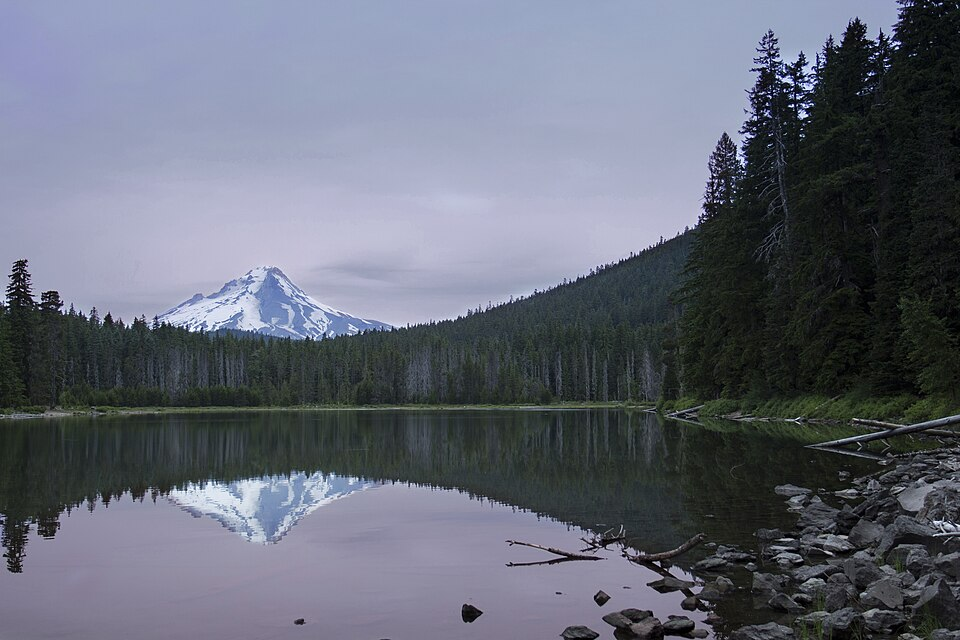
\includegraphics[width=0.75\linewidth]{example.jpg}
		\caption{An example figure.}
		\label{fig:example}
	\end{figure}
	
	Figure references can be written with \verb|\ref| or, preferably, \verb|\cref|. For example, \cref{fig:example} automatically includes the appropriate reference name.
	
	LaTeX{} will determine a suitable float position according to the surrounding text and the placement options supplied to the environment.
	
	
	\subsection{How to Add Tables}
	
	Use the \texttt{table} and \texttt{tabular} environments for tables. The template includes \texttt{booktabs}, so \verb|\toprule|, \verb|\midrule|, and \verb|\bottomrule| are available.
	
	\begin{table}[t]
		\centering
		\caption{An example table.}
		\label{tab:example}
		\begin{tabular}{lcc}
			\toprule
			Method & Metric 1 & Metric 2 \\
			\midrule
			Baseline & 0.00 & 0.00 \\
			Proposed method & 0.00 & 0.00 \\
			\bottomrule
		\end{tabular}
	\end{table}
	
	For example, \cref{tab:example} refers to the table above.
	
	
	\subsection{How to Add Comments}
	
	Anything following the \verb|%| symbol on a line is treated as a comment and is not typeset in the document.
	
	For example:
	
	\begin{verbatim}
		% This line is a comment.
		This line appears in the document.
	\end{verbatim}
	
	Comments are useful for reminders, alternative wording, implementation notes, or temporarily disabling parts of the source file.
	
	
	\subsection{How to Add Lists}
	
	Numbered lists can be created with the \texttt{enumerate} environment:
	
	\begin{enumerate}
		\item First item.
		\item Second item.
	\end{enumerate}
	
	Bullet lists can be created with the \texttt{itemize} environment:
	
	\begin{itemize}
		\item First item.
		\item Second item.
	\end{itemize}
	
	
	\subsection{How to Write Mathematics}
	
	Inline mathematics is enclosed by \verb|$...$|. Displayed equations can be written with environments such as \texttt{equation}.
	
	Let $X_1, X_2, \ldots, X_n$ be independent and identically distributed random variables with $\mathbb{E}[X_i] = \mu$ and $\mathrm{Var}[X_i] = \sigma^2 < \infty$. Define
	
	\begin{equation}
		S_n = \frac{X_1 + X_2 + \cdots + X_n}{n}
		= \frac{1}{n}\sum_{i=1}^{n} X_i.
		\label{eq:sample-mean}
	\end{equation}
	
	Then \cref{eq:sample-mean} gives the sample mean.
	
	Reusable mathematical commands and notation can be placed in \texttt{math\_commands.tex} so that they can be used consistently throughout the paper.
	
	
	\subsection{How to Write Theorems}
	
	The template provides commonly used theorem environments, including \texttt{theorem}, \texttt{property}, \texttt{proposition}, \texttt{lemma}, \texttt{corollary}, \texttt{definition}, \texttt{assumption}, \texttt{remark}, and \texttt{conjecture}.
	
	For example:
	
	\begin{theorem}
		\label{thm:example}
		For any $a,b \in \mathbb{R}$,
		\[
		(a+b)^2 = a^2 + 2ab + b^2.
		\]
	\end{theorem}
	
	Theorem environments can be referenced in the same way as equations, figures, and tables. For example, \cref{thm:example} refers to the theorem above.
	
	Definitions, lemmas, propositions, and other theorem-like environments can be written similarly:
	
	\begin{definition}
		\label{def:convergence}
		A sequence $(x_n)$ is said to converge to $x$ if, for every
		$\varepsilon > 0$, there exists $N$ such that
		\[
		|x_n - x| < \varepsilon
		\]
		for all $n \geq N$.
	\end{definition}
	
	For example, \cref{def:convergence} gives a definition using the same numbering system.
	
	
	\subsection{How to Use Cross-References}
	
	Add a \verb|\label| to sections, equations, figures, tables, algorithms, theorem environments, and other numbered objects. They can then be referenced with \verb|\ref| or \verb|\cref|.
	
	For example:
	
	\begin{verbatim}
		\section{Method}
		\label{sec:method}
		
		See \cref{sec:method}.
	\end{verbatim}
	
	The template loads \texttt{cleveref}, which automatically inserts the appropriate object name when \verb|\cref| or \verb|\Cref| is used.
	
	
	\subsection{How to Add Citations and References}
	
	Bibliographic entries should be stored in \texttt{references.bib}. The template uses \texttt{natbib} with numerical citations. The command \verb|\citep| produces a numerical citation such as \citep{greenwade93}, while \verb|\citet| includes the author name, as in \citet{greenwade93}.
	
	Other common bibliography types work in exactly the same way. A conference paper can be cited as \citep{exampleconference2026}, a book as \citep{examplebook2026}, a book chapter as \citep{examplechapter2026}, a technical report as \citep{examplereport2026}, and a preprint as \citep{examplepreprint2026}.
	
	Multiple references can also be cited together:
	
	\begin{verbatim}
		\citep{greenwade93,exampleconference2026,examplebook2026}
	\end{verbatim}
	
	The corresponding BibTeX entries are stored in \texttt{references.bib}. Replace the example entries with the references used by your paper.
	
	
	\subsection{How to Use Algorithms}
	
	The template provides the \texttt{algorithm} and \texttt{algpseudocode} packages.
	
	A minimal example is:
	
	\begin{algorithm}[t]
		\caption{Example Algorithm}
		\label{alg:example}
		\begin{algorithmic}[1]
			\Require Input $x$
			\Ensure Output $y$
			\State Initialize $y$
			\State Update $y$ using $x$
			\State \Return $y$
		\end{algorithmic}
	\end{algorithm}
	
	The algorithm can then be referenced as \cref{alg:example}.
	
	
	\subsection{How to Adjust the Template}
	
	General formatting settings such as page layout, typography, title formatting, section styles, float behavior, theorem environments, and author formatting are defined in \texttt{template.sty}.
	
	Reusable mathematical commands and notation can be placed in \texttt{math\_commands.tex}.
	
	Content specific to the paper should normally remain in \texttt{main.tex}, while bibliography entries belong in \texttt{references.bib}.
	
	Keeping these responsibilities separate makes the template easier to reuse and maintain.
	
	
	% ============================================================
	% References
	% ============================================================
	
	\bibliographystyle{plainnat}
	\bibliography{references}
	
	
	% ============================================================
	% Appendix
	% ============================================================
	%
	% Uncomment the following lines when an appendix is needed.
	% The template automatically inserts an appendix-only table of contents
	% after \appendix.
	%
	% \newpage
	% \appendix
	%
	% \section{Additional Details}
	%
	% Additional material goes here.
	%
	% \section{Additional Results}
	%
	% Additional material goes here.
	
	
\end{document}

